%!TEX TS-program = pdflatex
%!TEX root = ../main.tex
%!TEX encoding = UTF-8 Unicode


\section{Application}

\subsection{System design}

\begin{frame}{Use Case Diagram}
	The first step of our development to identify the use cases of our system.
	We have identified four main use cases:

	\begin{figure}[h!]
		\centering
		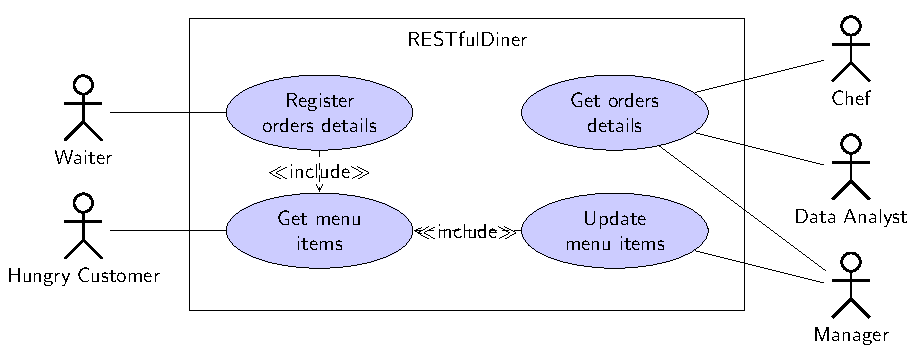
\includegraphics[width=0.9\textwidth,height=0.55\textheight,keepaspectratio]{images/usecases}
		\vspace*{-1\baselineskip}
		\caption{Use cases diagram}
		\label{fig:usecases}
	\end{figure}

\end{frame}

\begin{frame}{E/R Diagram}
	Next, the E/R diagram was designed to represent the data model of the
	system:

	\begin{figure}[h!]
		\centering
		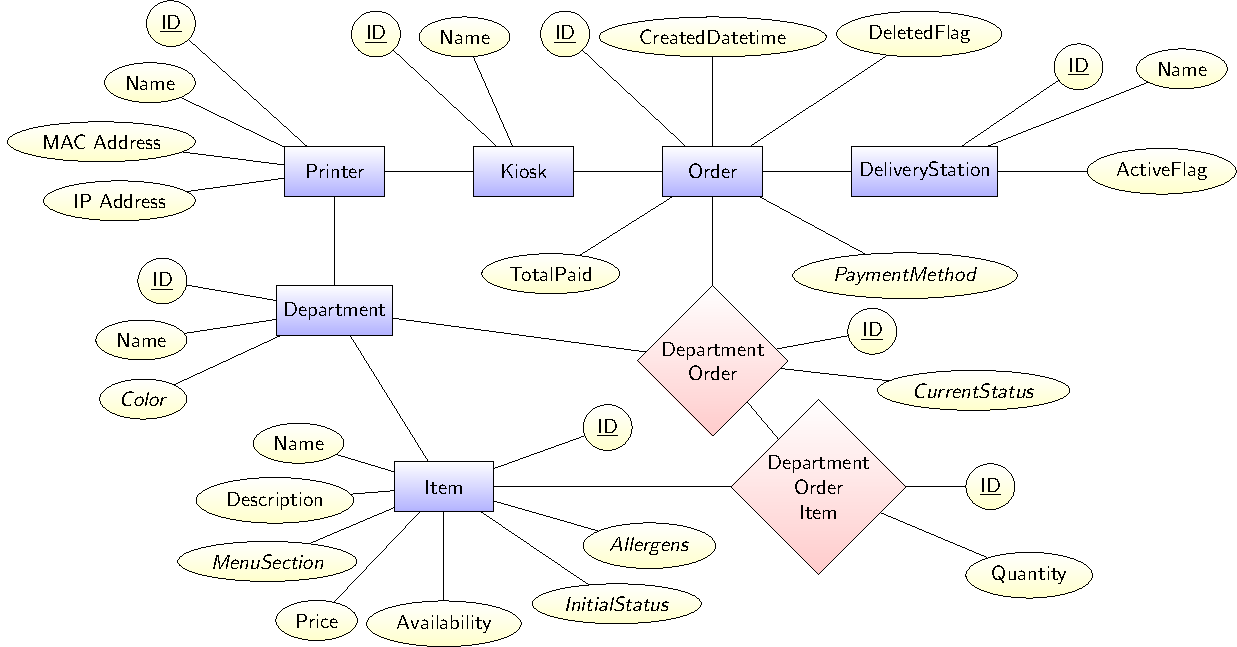
\includegraphics[width=\textwidth,height=0.57\textheight,keepaspectratio]{images/er}
		\caption{E/R diagram}
		\label{fig:er}
	\end{figure}

\end{frame}

\subsection{System implementation}

\begin{frame}[allowframebreaks]{Data model (logical) implementation}

	The data model has been implemented using the SQLAlchemy ORM, which
	provides a high-level interface to the (PostgreSQL, in this case) database.

	\lstinputlisting[language=PythonPlus,linerange={14-27}]{../app/models/_base.py}

	Any class inherits from the \texttt{BaseModel} class and is automatically
	mapped to a table in the database.

	\framebreak

	\vspace*{-1\baselineskip}
	\lstinputlisting[language=PythonPlus,linerange={13-33}]{../app/models/department.py}

\end{frame}

\begin{frame}[fragile]{Data model (physical) implementation}

	Since we are using an ORM, the physical implementation of the data model is
	automatically generated by the ORM itself.
	This is, for example, the code for the \texttt{department} table:
	
	\begin{lstlisting}[language=SQL]
CREATE TABLE department (
	id UUID NOT NULL,
	name VARCHAR(63) NOT NULL,
	color VARCHAR(63),
	printer__id UUID,
	PRIMARY KEY (id),
	UNIQUE (name),
	FOREIGN KEY(printer__id) REFERENCES printer (id)
);
COMMENT ON COLUMN department.id IS 'Unique Department instance identifier';
COMMENT ON COLUMN department.name IS 'Unique name of the department';
COMMENT ON COLUMN department.color IS 'A color between the Recognized color keyword names. See also https://www.w3.org/TR/SVG11/types.html#ColorKeywords';
COMMENT ON COLUMN department.printer__id IS 'Identifier of the printer the department is equipped with';\end{lstlisting}

\end{frame}

\begin{frame}[allowframebreaks,fragile]{API resources}
	The RESTful API has been implemented using the Flask web framework.

	\lstinputlisting[language=PythonPlus,linerange={12-12,16-31}]{../app/resources/department.py}

	\framebreak

	\vspace*{-1\baselineskip}
	\begin{lstlisting}
{
	"@context": {
		"schema": "https://schema.org/",
		"self": "@id",
		"type": "@type",
		"name": "schema:name",
		"printer": {
			"@id": "schema:isRelatedTo",
			"@type": "@id"
		},
		"license": {
			"@id": "schema:license",
			"@type": "@id"
		}
	},
	"license": "https://creativecommons.org/licenses/by/4.0/",
	"data": {
		"self": "http://127.0.0.1:5000/api/v1/departments/5b11618c-51f5-8000-8000-6496d5c5c0cf",
		"type": "schema:Organization",
		"name": "Kitchen",
		"printer": "http://127.0.0.1:5000/api/v1/printers/5b11618c-51f5-8000-8000-2a5553677712"
	}
}\end{lstlisting}
		
\end{frame}

\begin{frame}{Demo}
	A live demo of the system is available at \url{https://diner.enricostefanel.it}.

	\begin{figure}
		\centering
		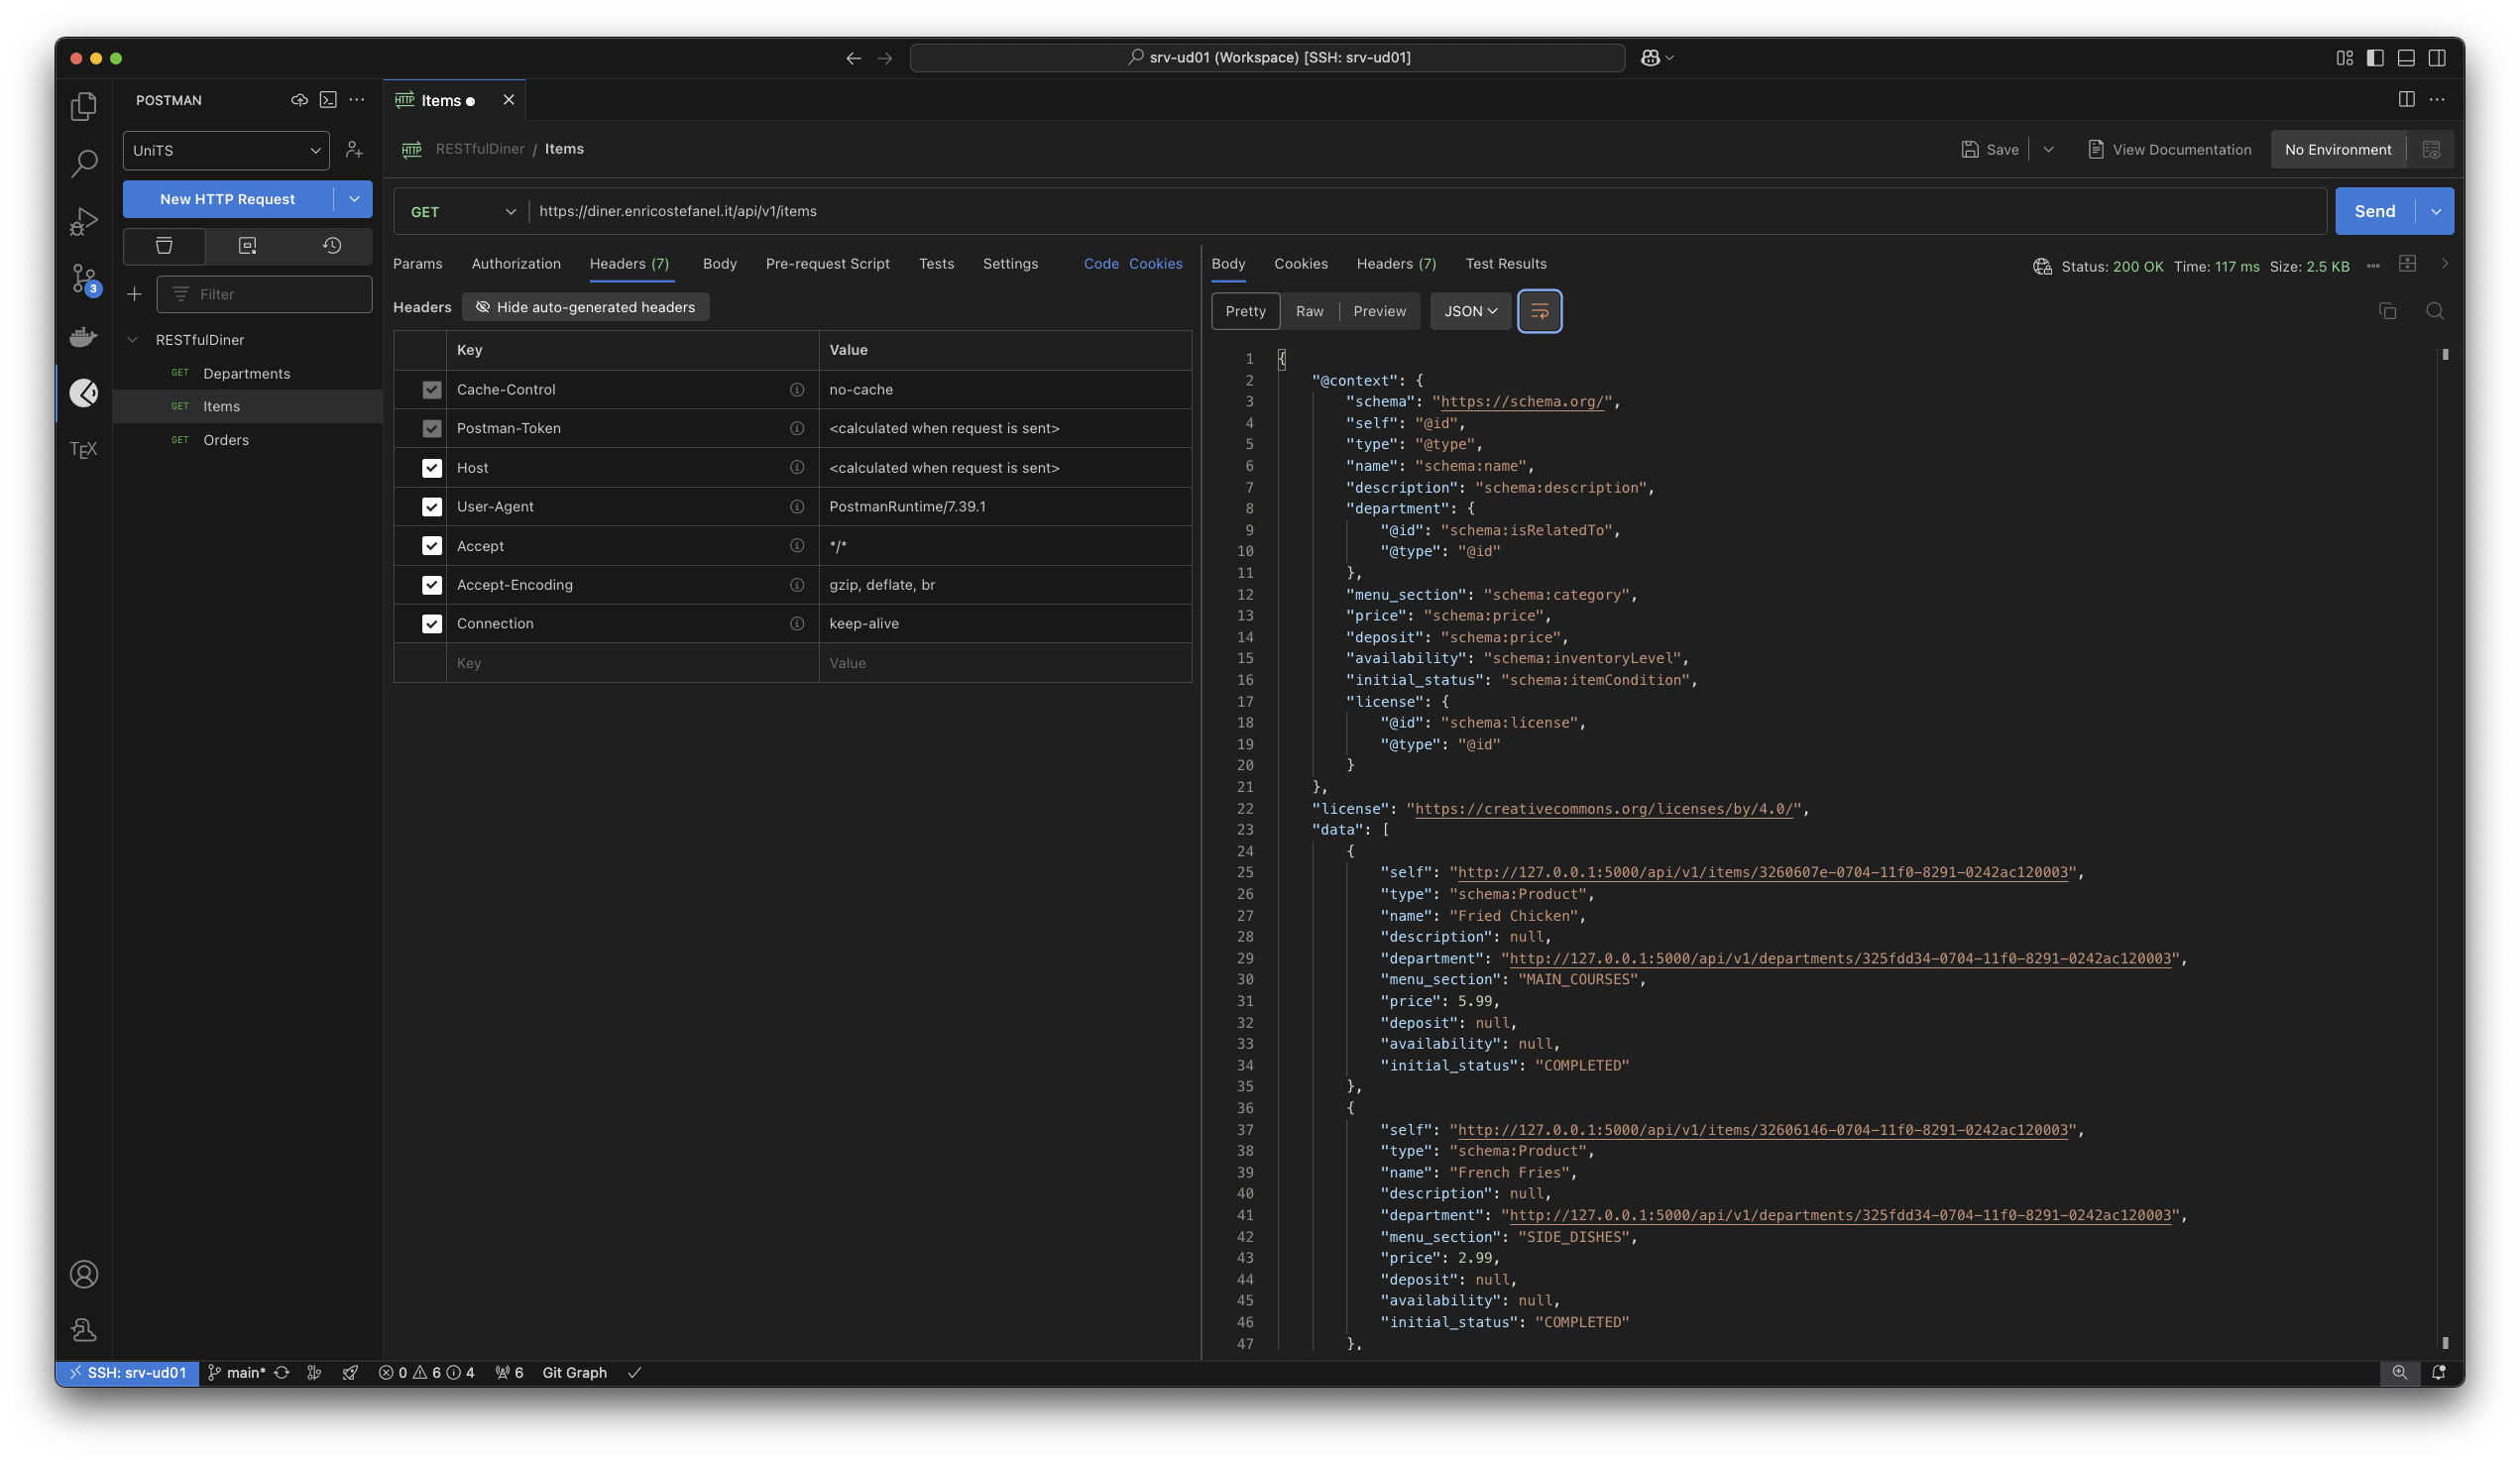
\includegraphics[width=0.9\textwidth,height=0.6\textheight,keepaspectratio]{images/postman.png}
		\vspace*{-1\baselineskip}
		\caption{Demo of the system using Postman}
		\label{fig:demo}
	\end{figure}
\end{frame}


\section{Open Data principles}

\subsection{Linked Open Data}

\begin{frame}[allowframebreaks]{Linked Open Data\autocite{Berners-Lee_2006} requirements}
	\begin{block}{\faStar\faStarO\faStarO\faStarO\faStarO}
		Make your stuff available on the Web (whatever format) under an open
		license.
	\end{block}
	\vspace*{-8pt}
	\begin{block}{\faStar\faStar\faStarO\faStarO\faStarO}
		Make it available as structured data (e.g., Excel instead of image scan
		of a table).
	\end{block}
	\vspace*{-8pt}
	\begin{block}{\faStar\faStar\faStar\faStarO\faStarO}
		Make it available in a non-proprietary open format (e.g., CSV instead of
		Excel).
	\end{block}
	These requirements are satisfied by our RESTful API that allows
	publicly access to data in JSON-LD\autocite{Sporny_2014} format and provide
	them under Creative Commons license.

	\framebreak

	\begin{block}{\faStar\faStar\faStar\faStar\faStarO}
		Use URIs to denote things, so that people can point at your stuff.
	\end{block}
	\vspace*{-8pt}
	\begin{block}{\faStar\faStar\faStar\faStar\faStar}
		Link your data to \textcolor{UNITSCherry}{other} data to provide context.
	\end{block}
	Every resource in the system is identified by a URI, and can be accessed
	by a simple HTTP GET request to that URI. A relation between resources
	is established by linking them in the JSON response.
	We are not fully inter-operable with other datasets, given the nature of the
	system, but we are open to the possibility of linking our data with
	other datasets in the future.
\end{frame}

\subsection{FAIR Data Principles}

\begin{frame}[allowframebreaks]{FAIR\autocite{Wilkinson_2016} principles requirements}
	\begin{block}{Findable}
		\begin{itemize}
			\item \textbf{F1.} (Meta)data are assigned a globally unique and persistent identifier
			\item \textbf{F2.} Data are described with rich metadata (defined by R1 below)
			\item \textcolor{UNITSCherry}{\textbf{F3.} Metadata clearly and explicitly include the identifier of the data they describe}
			\item \textcolor{UNITSCherry}{\textbf{F4.} (Meta)data are registered or indexed in a searchable resource}
		\end{itemize}
	\end{block}

	The JSON-LD data representation includes the URI of the resource itself and the related resources.
	Since the metadata is provided together with the data, there is no need to include
	the identifier of the data in the metadata.
	
	\framebreak

	\begin{block}{Accessible}
		\begin{itemize}
			\item \textbf{A1.} (Meta)data are retrievable by their identifier using a standardized communications protocol
			\item \textbf{A1.1} The protocol is open, free, and universally implementable
			\item \textbf{A1.2} The protocol allows for an authentication and authorization procedure, where necessary
			\item \textcolor{UNITSCherry}{\textbf{A2.} Metadata are accessible, even when the data are no longer available}
		\end{itemize}
	\end{block}

	The HTTP protocol ensured that (meta)data is freely accessible, allowing for an
	authorization procedure where necessary (e.g.,\texttt{POST} operations).
	
	\framebreak
	
	\begin{block}{Interoperable}
		\begin{itemize}
			\item \textbf{I1.} (Meta)data use a formal, accessible, shared, and broadly applicable language for knowledge representation
			\item \textbf{I2.} (Meta)data use vocabularies that follow FAIR principles
			\item \textcolor{UNITSCherry}{\textbf{I3.} (Meta)data include qualified references to other (meta)data}
		\end{itemize}
	\end{block}
	
	\framebreak
	
	\begin{block}{Reusable}
		\begin{itemize}
			\item \textbf{R1.} Meta(data) are richly described with a plurality of accurate and relevant attributes
			\item \textbf{R1.1} (Meta)data are released with a clear and accessible data usage license
			\item \textcolor{UNITSCherry}{\textbf{R1.2} (Meta)data are associated with detailed provenance}
			\item \textcolor{UNITSCherry}{\textbf{R1.3} (Meta)data meet domain-relevant community standards}
		\end{itemize}
	\end{block}
\end{frame}


\section{Data Infrastructure}

\subsection{Data Management}

\begin{frame}[allowframebreaks]{Data Management Plan}

	\begin{enumerate}\justifying
		\item \textbf{How will the data be \textcolor{UNITSCherry}{created}?} The data will be created by the
		      restaurant staff, who will use the system to manage the restaurant's
		      departments, tables, and printers.
		\item \textbf{How will the data be \textcolor{UNITSCherry}{documented}?} The data will be documented in
		      the system's database, and the API will provide a JSON-LD representation of
		      the data.
		\item \textbf{Who will \textcolor{UNITSCherry}{access} the data?} The data will be publicly accessible
		      through the RESTful API.
		\item \textbf{How will the data be \textcolor{UNITSCherry}{stored}?} The data will be stored by the
		      system's database, which is a PostgreSQL database. In case, the database
			  can also be installed on a cloud service.
		\item \textbf{How will the data be \textcolor{UNITSCherry}{shared}?} The data will be shared through the
		      RESTful API, which will provide a JSON-LD representation of the data for
			  basic HTTP requests (GET, POST, PUT, DELETE).
		\item \textbf{How will the data be \textcolor{UNITSCherry}{preserved}?} The data will be preserved by
		      the system's database, which will be backed up regularly to ensure data
			  integrity.
		\item \textbf{Who will \textcolor{UNITSCherry}{back up} the data?} The data will be backed up by the
		      system administrator, who will ensure that the database is backed up
			  regularly.
	\end{enumerate}
\end{frame}

\subsection{Storage and Backup}

\begin{frame}[allowframebreaks]{Storage metrics}
	Let's try to imagine some storage metrics for our system:

	\begin{itemize}
		\item \textbf{Bandwidth} (volume of data read and written in a second):
		\begin{itemize}
			\item{\textbf{How many orders per day?} About 200 orders per day, which %
			means less than a order per minute.}
			\item{\textbf{How many items per order?} An average of 5 items per order %
			can be considered a good approximation.}
		  \end{itemize}
		We are talking about less than 1 MB of data per day, which is not a big deal
		for a modern database. $\rightarrow$ \textcolor{UNITSBlue}{We do not need a %
		distributed database, a single instance is enough.}
		\item \textbf{Latency} (time taken to read and write data): since the system does %
		not imply heavy computation and it is not required to guarantee real-time %
		responses, we can assume that the latency is not a big deal. A good %
		approximation is that the latency is less than 1 second for a single %
		request. $\rightarrow$ \textcolor{UNITSBlue}{Even an infrastructure based on %
		hard disk drives is fast enough  for our purpose.}
		\item \textbf{Scalability} (ability to handle increasing load): the system could, %
		in theory, be designed to already foreseen a future increase in the number of %
		users and restaurants. $\rightarrow$ \textcolor{UNITSBlue}{We can use a cloud %
		service to host the database in future, which can be easily scaled up or down. %
		The migration will be easy and fast, and the API will only require to change the %
		connection string to the new database.}
		\item \textbf{Reliability} (ability to recover from failures): since we are using %
		the system in a running business, it is strictly required to have a %
		reliable system. The database must be backed up regularly to ensure data %
		integrity. $\rightarrow$ \textcolor{UNITSBlue}{We can use a cloud service to host %
		the database, which can be easily backed up and restored in case of failure. Furthermore, %
		the filesystem could be based on a RAID 1 configuration, which assures the replication %
		of the data on two different disks and rapid recovery in case of failure.}
	\end{itemize}

\end{frame}
